\chapter{Google Cardboard AR demo}
\label{chp:Google Cardboard AR demo}

Having AR in place it needs to be tweaked to achieve the so called stereoscopic effect. The last produced application and all need files from chapter \ref{chp:AR Library} are copied into the file structure from this chapter and {markerController.html} will serve as base code and be called \textit{fullscreen.html}.

\section{Fullscreen}
\label{sec:fullscreen}

It could be surprising that it is not that simple to get the browser to go to fullscreen. Due to controlling reasons most browsers do not allow the automatic fully programmatic switch to fullscreen. It has to be the user that invokes the request directly by clicking an element that will trigger it. To provide this button the in section \ref{sec:enhancedScene} from the previous chapter added {dat.GUI} provides the button and the actual function. Adding the panel, the setting and attaching the function as described in the w3schools tutorial at \url{https://www.w3schools.com/howto/howto_js_fullscreen.asp}.


\section{Stereoscopic View}

To evolve the display further \textit{stereoscopicView.html} was created out of  \textit{fullscreen.html}. Everything other in place this is the step to convert a simple AR-application into the Google Cardboard supporting one. Therefore it is recommended to have the Google Cardboard - enhanced with a hole for the camera - ready and checking for bright lighting condition for the marker.

Despite the existence of the example of the stereoscopic effect given in the \textit{Awe.js} ZIP-Archive it is not quite clear whether this feature will get along with the existing application. There are other dependencies and another loading order used. To get the stereo view applied in the current application there are just a view adaptations to do:
\begin{itemize}
\item \textit{third-party/plugins/StereoEffect.js} has to be listed in \textit{files} of \textit{awe.util.require}
\item add \textit{rotation: \{ x:0, y:180, z:180 \}} and  \textit{position: \{ x:0, y:0, z:-250 \}} to the \textit{jsartoolkit\_marker\_64} poi
\item add \textit{awe.settings.update(\{data:\{value: 'stereo'\}, where:\{id: 'view\_count'\}\});}
\item comment out \textit{awe.plugins.view('jsartoolkit').enable();}
\end{itemize}

after those four simple steps  the split screen shows up for the stereoscopic effect. However by commenting out the \textit{jsartoolkit} plugin, the marker recognition is disabled. It looks like those two functionality are mutually exclusive. That would mean, that it is not possible to build an AR stereoscopic application with \textit{Awe.js}.

The first approach to find a solution by reordering of code lines - in hope to manipulate the loading - does not work. 
Enable \textit{jsartoolkit} again and play around manually with unregister, register, enable and disable the plugin - this can be done with the GUI panel - leads to an interesting observation. The unregistration of the plugin will start the splitt view. However the followed reregistration of \textit{jsartoolkit} the objects are not placed on the marker - not even showed on the screen - the \textit{animate} function that was created in the previous chapter in section \ref{sec:markerController} seems still to get the marker information.

As the provided solution breaks but the marker detection still seems to work it should be possible to create a workaround that will be put in place in the \textit{workaround.html}.

\section{Workaround}
\label{sec:workaround}

Using \textit{Three.js} to convert the retrieved matrix into rotation, position and scaling it shows, that something got screwed up with the coordinate system amusingly when the stereoscopic cameras come into place. Instead of tweaking the third-party code - that the console message tells that a function is deprecated - I will work with the provided data from the marker recognition. This could give additional control to stabilize the projected object. 

First the second poi that served as parent node for the other projections can easily be loosed from the actual marker and be feed in the modified data from the marker and be updatet over the \textit{Awe.js} API. The data have to be modified as follows:
\begin{itemize}
\item In the position the z coordinate got flipped around the origin. Switching the sign will do the work.
\item As the \textit{Three.js} function converting the matrix into rotations returns radians the values has to be divided by pi and multiplied by 180 to get the from \textit{Awe.js}  demanded degrees for the rotation update.
\item Further all axis rotation are inverted that can be redone by switching the sign.
\end{itemize}
It shows, that the scaling could be done too however is not needed. 
To get the exact same behaviour as in the section \ref{sec:fullscreen} it is important, that the poi does not only get updated with position and rotation but also with the visibility. Being able to even influence when the poi is shown it is already better to control as the indented implementation as smooth transitions could be made. This approach - what is more important - allows to start the stereoscopic view together with the marker recognition. To do so, the recognition plugin has to be unregistered and as soon as the split view starts be registered to use it again. This process could be done fully automatically without the user having to do anything - beside the toggling of the fullscreen - but I like leaving the freedom to the user decide when to switch the mode. Figure \ref{fig:workaround} show everything - fullscreen, stereoscopic effect, marker detection and marker as controller - combined when running workaround.html.  

\begin{figure}[h]
    \centering
    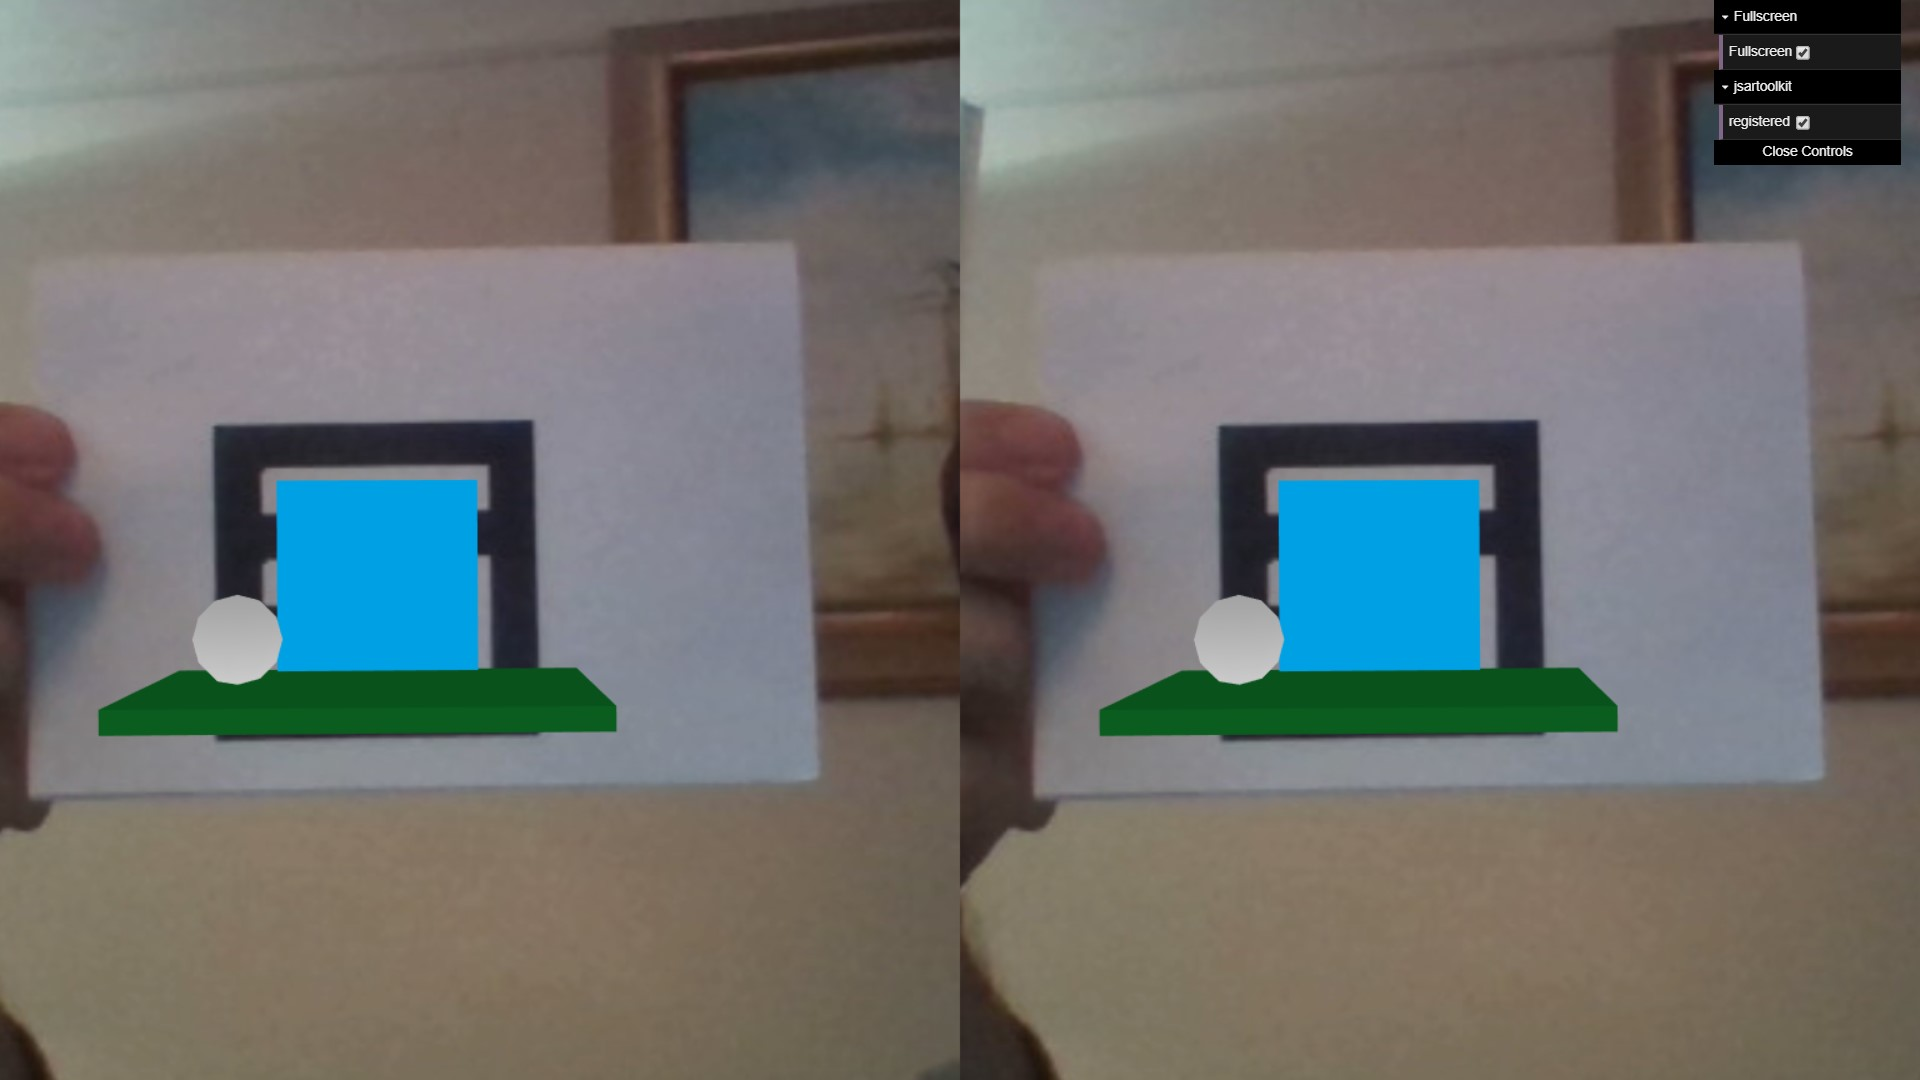
\includegraphics[height=5cm]{Document/Figures/chapter4/ScreenshotWorkaroundFullStereo.jpg}
    \caption[Screenshot workaround]{Screenshot of workaround in fullscreen an stereo view when  running \mbox{\textit{workaround.html}}}
    \label{fig:workaround}
\end{figure}



\section{Final Demo}

The final demon is in the HTML file \textit{finalDemo.html}.

Small aesthetic changes like placing the ball a little lower or let the \textit{Loading...} appear a bit bigger are applied. To make the switching to split screen for the stereoscopic effect easier for the user I added a single button to the control panel that will do the switching of and on of the plugin to start the split view. 
To make sure that no actions are invoked by the user too early before the key parts are loaded and ready the control panel is loaded when everything else is ready too and therefore only then will be displayed on the screen.

Enhancing the scene by adding playful elements such as a tree that can grow or be run over by the ball steered by the user. In the later case the tree will start to grow randomly on another place. The tree is basically just a cylinder. The \textit{Awe.js} API allows to create elements as in \textit{Three.js} like the cylinder described at \url{https://threejs.org/docs/\#api/en/geometries/CylinderGeometry}.

Adding further controls to the panel the user can resize the playground width with a slider or changing the animation growth time of the tree. The later - by the way - is a nice feature of \textit{Awe.js} update function that allows to set a duration time over which the update will linearly be spread.

A screenshot of the final demo running \textit{finalDemo.html} is shown in figure \ref{fig:finalDemo}. This application can either run locally meaning that the files can be called by their path in the browser. When transferring and copying the files to the smartphone it can be tricky to find their local path. 

Another way to provide the files to the browser is to run them on a server. Because of security reasons for some of the used function and APIs the server has to be the localhost or using HTTPS.

When the file is called it can take some times to load. It will also not be directly in the final mode to view it in the Google Cardboard. First the fullscreen as to be activated manually as described in section \ref{sec:fullscreen} and the split view to enable the stereoscopic effect needs also to be activated like written above in this section for reasons explained in section \ref{sec:workaround}. To minimize the control panel it can be closed before inserting the smartphone into the Google Camera.

It has also to be taken in account that when the device camera lies on the same side as the screen that the presented image can react contraintuitive to the movements of the user as it does not behave like a mirror. Even so the picture is processed and calculated correctly. 

\begin{figure}[h]
    \centering
    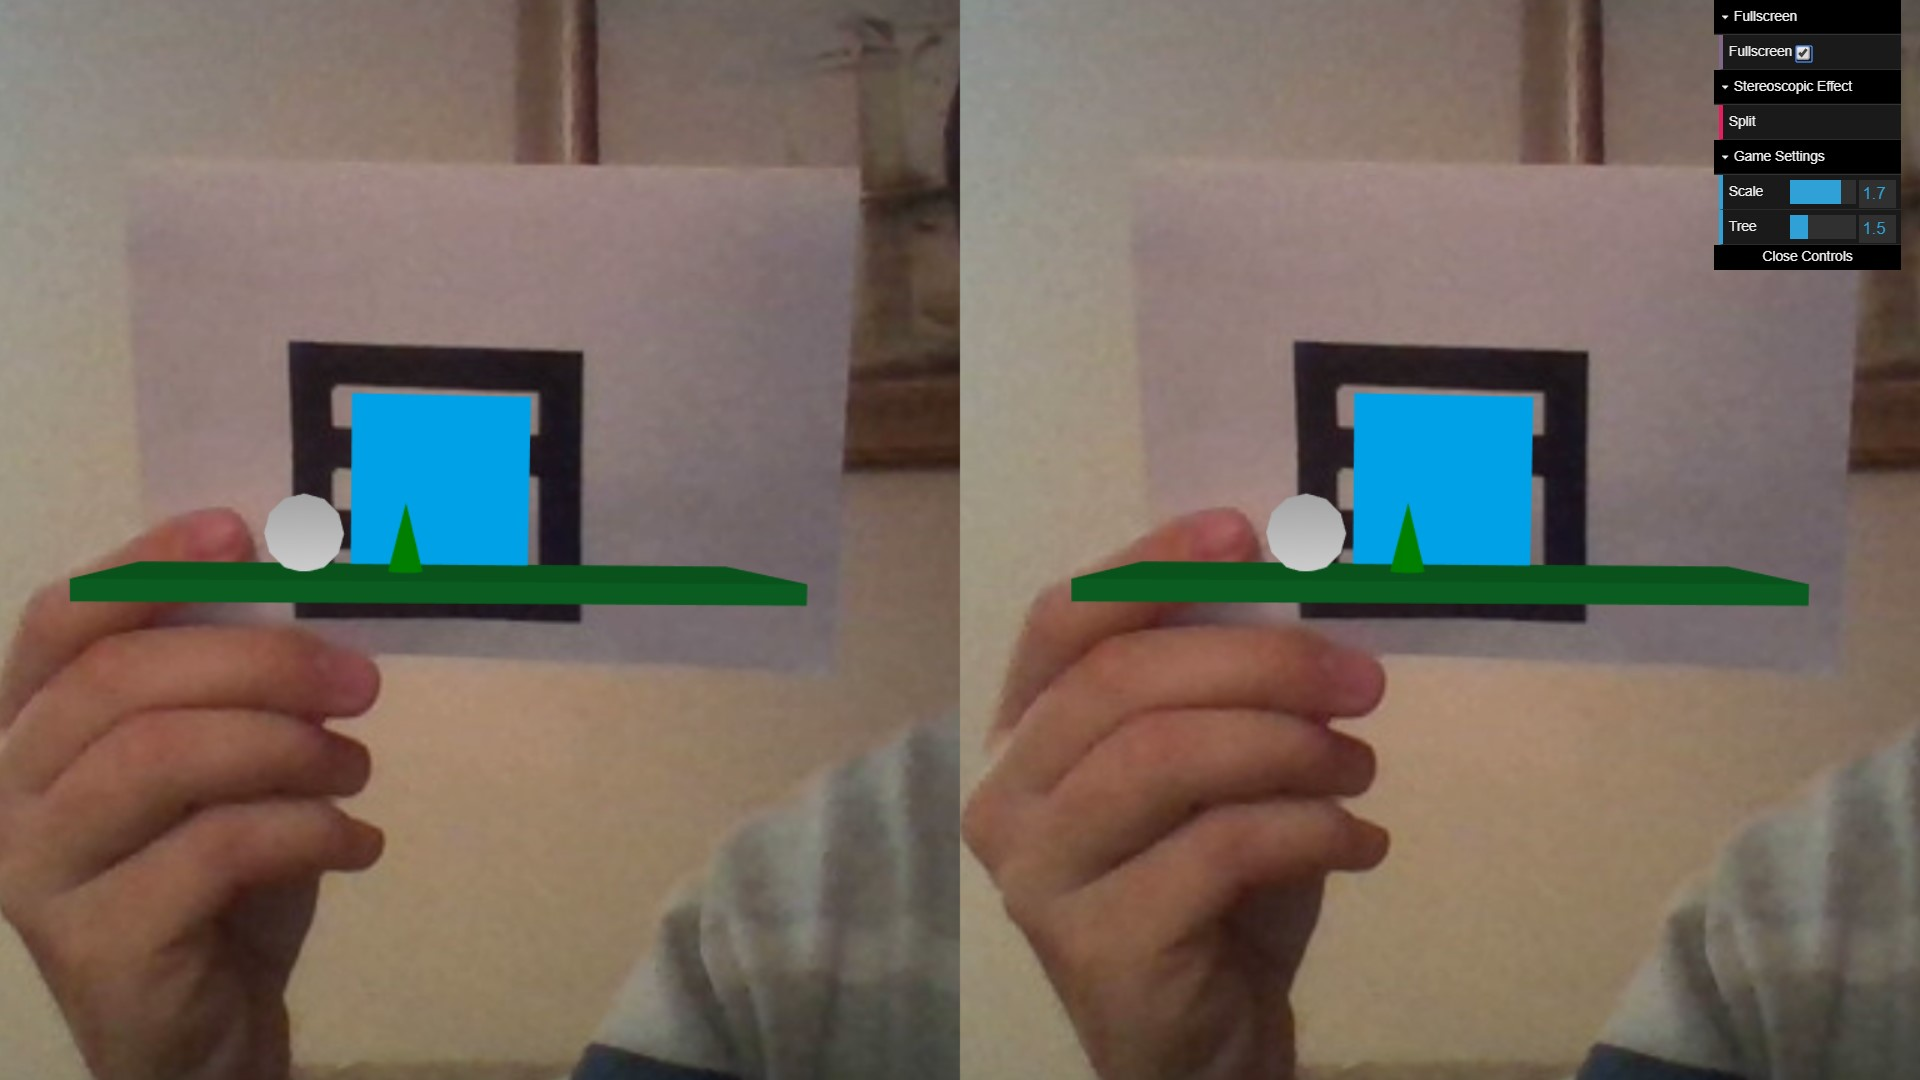
\includegraphics[height=5cm]{Document/Figures/chapter4/ScreenshotFinalDemo.jpg}
    \caption[Screenshot final demo]{Screenshot of final demo running \mbox{\textit{finalDemo.html}}}
    \label{fig:finalDemo}
\end{figure}


\section{Evaluation}
extend put keep it small

split screen could be differently
everything done without changing third-party code

gyro would be possible


assumed that head is straight and looks at the marker which will be placed parallel to the users face such as it would be placed on a wall or in a book or magazine. 